\subsection{Profiling with the pbdPROF Package}
\makesubcontentsslidessec


\begin{frame}
  \begin{block}{Introduction to \textbf{pbdPROF}}
    \begin{itemize}
    \item Successful Google Summer of Code 2013 project.
    \item Available on the CRAN.
    \item Enables profiling of MPI-using R scripts (+).
    \item Also reads, parses, and plots profiler outputs.
    \end{itemize}
  \end{block}
\end{frame}


\begin{frame}
  \begin{block}{How it works}
    MPI calls get hijacked by profiler and logged:
    \begin{center}
      \hspace{2cm}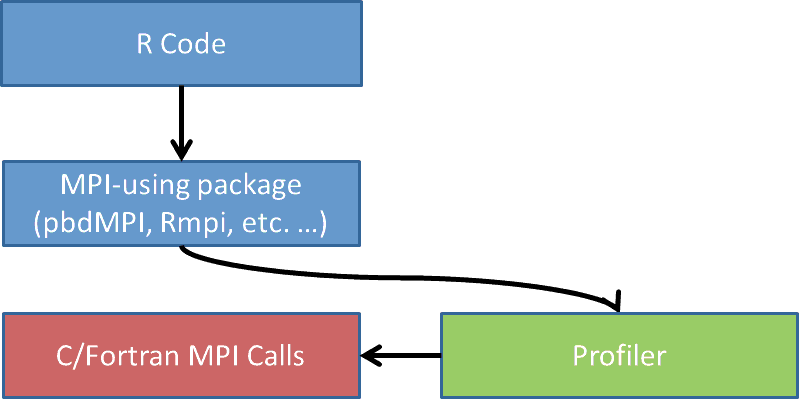
\includegraphics[width=0.8\textwidth]{../common/pics/prof/mpi_profiler}
    \end{center}
  \end{block}
\end{frame}


\begin{frame}
  \begin{block}{Introduction to \textbf{pbdPROF}}
    \begin{itemize}
    \item Currently supports the profilers \textbf{fpmpi} and \textbf{mpiP}.
    \item \textbf{fpmpi} is distributed with \textbf{pbdPROF} and
      installs easily, but offers minimal profiling capabilities.
    \item \textbf{mpiP} is fully supported also, but you have to
      install and link it yourself.
    \end{itemize}
  \end{block}
\end{frame}
